% Relatório do laboratório 3 de servo
% Felipe Bandeira da Silva
% 09/06/2013

%\documentclass[a4paper, 10pt]{article}
\documentclass[paper=a4, fontsize=11pt]{article}

\usepackage[framed,numbered,autolinebreaks,useliterate]{mcode}

\usepackage[brazil]{babel}
\usepackage[utf8]{inputenc}
\usepackage{listings}
\usepackage{color}
\usepackage{amsthm}
\usepackage{graphicx}

\setlength{\parindent}{0pt}
\setlength{\parskip}{18pt}

\title{Relatório, Laboratório 4.\\Servo 1}
\author{Felipe Bandeira da Silva}


%%%%%%%%%%%%%%%%%%%%%%%%%%%%%%%%%%%%%%%%%%%%%%%%%%%%%%%%%%%%%%%%%%%%%%%%%%%%%%%%
% MAIN
%%%%%%%%%%%%%%%%%%%%%%%%%%%%%%%%%%%%%%%%%%%%%%%%%%%%%%%%%%%%%%%%%%%%%%%%%%%%%%%%

\begin{document}

%\maketitle

%\begin{abstract}
%Utilizar o Matlab para analisar a resposta transitória de sistemas de 1ª ordem
%ao degrau e estudar o efeito do controle proporcional sobre os aspectos de
%estabilidade, velocidade de resposta e erro em regime permanente.
%\end{abstract}


% ------------------------------------------------------------------------------
% LaTeX Template: Titlepage
% This is a title page template which be used for both articles and reports.
%
% Copyright: http://www.howtotex.com/
% Date: April 2011
% ------------------------------------------------------------------------------

% -------------------------------------------------------------------------------
% Preamble
% -------------------------------------------------------------------------------
%\documentclass[paper=a4, fontsize=11pt,twoside]{scrartcl}		% KOMA article

%\usepackage[a4paper,pdftex]{geometry}										% A4paper margins
%\setlength{\oddsidemargin}{5mm}												% Remove 'twosided' indentation
%\setlength{\evensidemargin}{5mm}

%\usepackage[english]{babel}
%\usepackage[protrusion=true,expansion=true]{microtype}	
%\usepackage{amsmath,amsfonts,amsthm,amssymb}
%\usepackage{graphicx}

% ------------------------------------------------------------------------------
% Definitions (do not change this)
% ------------------------------------------------------------------------------
\newcommand{\HRule}[1]{\rule{\linewidth}{#1}} 	% Horizontal rule

\makeatletter							% Title
\def\printtitle{%						
    {\centering \@title\par}}
\makeatother									

\makeatletter							% Author
\def\printauthor{%					
    {\centering \large \@author}}				
\makeatother							

% ------------------------------------------------------------------------------
% Metadata (Change this)
% ------------------------------------------------------------------------------
\title{	\normalsize \textsc{Universidade de Fortaleza} 	% Subtitle of the document
		 	\\[2.0cm]													% 2cm spacing
			\HRule{0.5pt} \\										% Upper rule
			\LARGE \textbf{\uppercase{Relatório 3\\Laboratório Servo 1}}	% Title
			\HRule{2pt} \\ [0.5cm]								% Lower rule + 0.5cm spacing
			\normalsize \today									% Todays date
		}

\author{
		Felipe Bandeira da Silva\\	
		Universidade de Fortaleza-UNIFOR\\	
		Engenharia Elétrica\\
        \texttt{felipeband18@gmail.com} \\
}


% ------------------------------------------------------------------------------
% Maketitle
% ------------------------------------------------------------------------------
\thispagestyle{empty}				% Remove page numbering on this page

\printtitle									% Print the title data as defined above
  	\vfill
\printauthor								% Print the author data as defined above
% ------------------------------------------------------------------------------
% Begin document
% ------------------------------------------------------------------------------

% ------------------------------------------------------------------------------
% End document
% ------------------------------------------------------------------------------



\newpage

%%%%%%%%%%%%%%%%%%%%%%%%%%%%%%%%%%%%%%%%%%%%%%%%%%%%%%%%%%%%%%%%%%%%%%%%%%%%%%%
% QUESTÃO 1
%%%%%%%%%%%%%%%%%%%%%%%%%%%%%%%%%%%%%%%%%%%%%%%%%%%%%%%%%%%%%%%%%%%%%%%%%%%%%%%
\section{Primeira questão}

O primeiro sistema físico é modelado com a equação 1
\begin{equation}
    G_1(s) = \frac{1}{s+1}
\end{equation}

A equação temporal da equação 1 quando submetida a um degrau unitário
é facilmente encontrada aplicando a transformada inversa de Laplace,

\begin{equation}
    G_1(s) = \frac{1}{s+1} \frac{1}{s}
\end{equation}

Aplicando o comando $residue$ em 2 para a expansão em frações parciais,

\begin{equation}
    G_1(s) = \frac{-1}{s+1} + \frac{1}{s}
\end{equation}

De 3 é possível encontrar a reposta temporal,

\begin{equation}
    g_1(t) = -e^{-t} + 1
\end{equation}

A plotagem do gráfico pode ser usada para a facilitar o visualização
do comportamento da função,

\begin{center}
    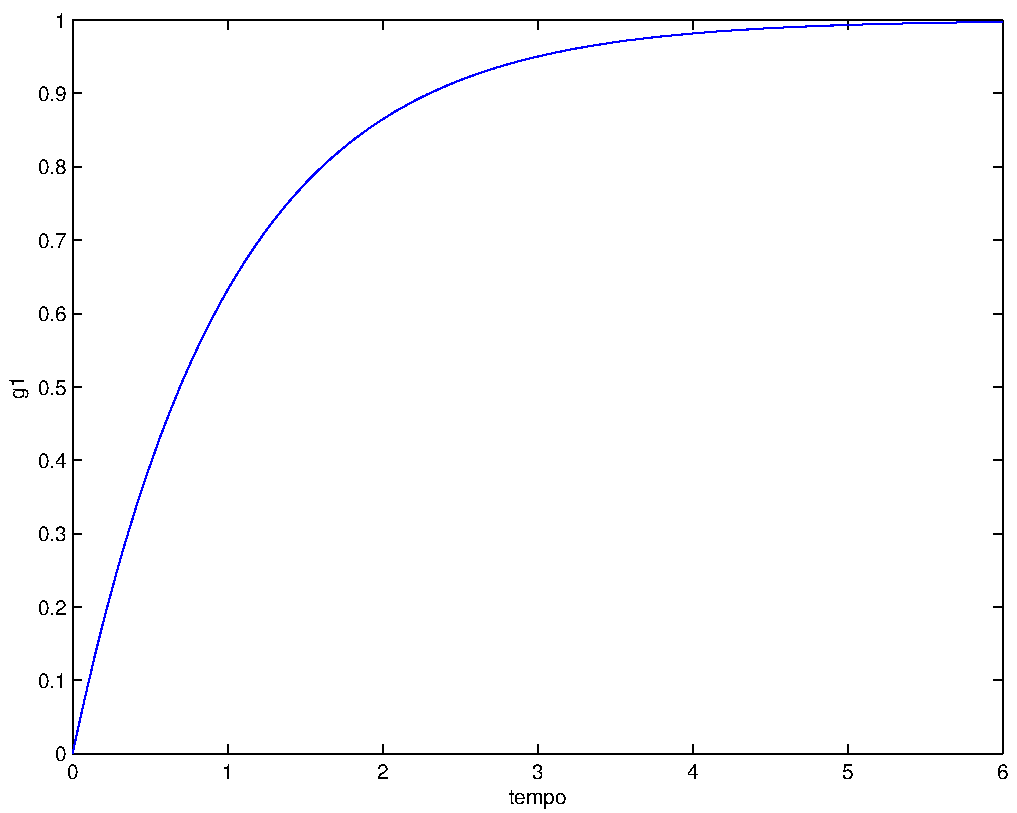
\includegraphics[scale=.5]{q1g1.pdf}
\end{center}

Por inspeção é possível notar que o sistema se estabiliza após um tempo
e seu valor em regimente permanente é 1. Mostrando que o sistema apresenta
uma estabilidade. Esta estabilidade pode ser melhor analisada plotando
a localização dos polos no plano-s.

\begin{center}
    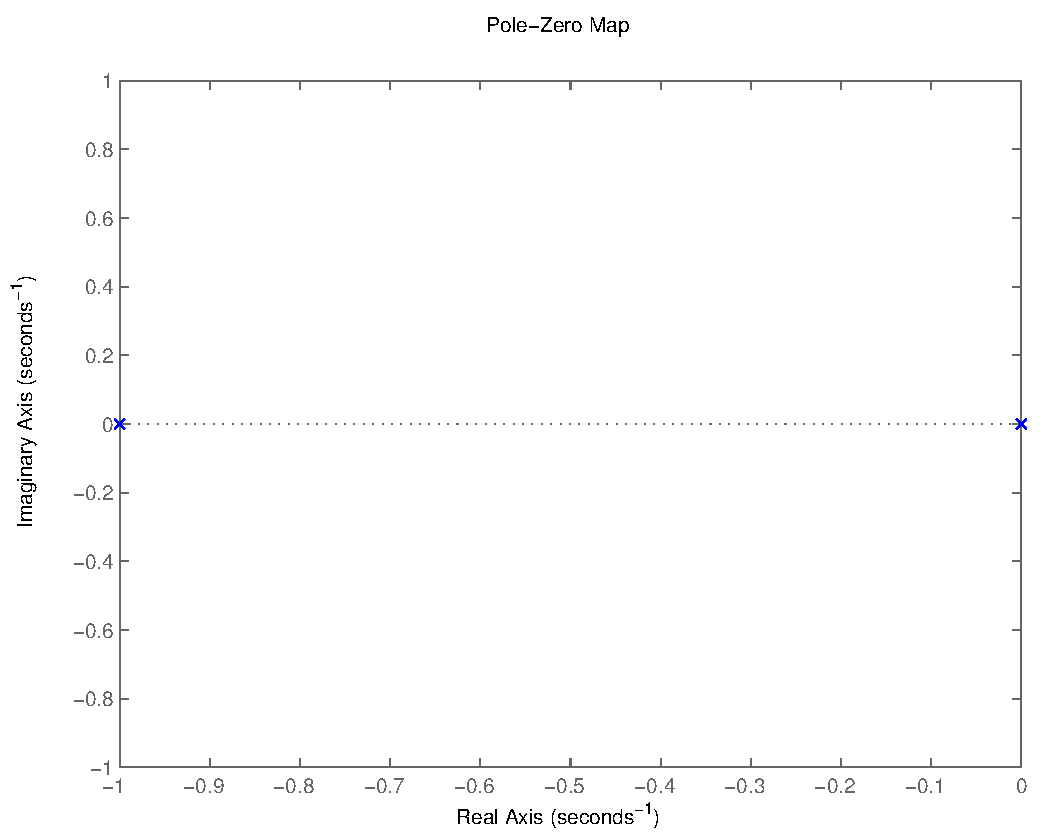
\includegraphics[scale=.5]{pzq1g1.pdf}
\end{center}

Como é possível observar existem dois polos no eixo real e com valores 
menor igual a zero, mostrando que o sistema é \textbf{estável}. Fato este
que está diretamente ligado a posição dos polos no eixo $\sigma$(eixo real).

Analisando agora a função,

\begin{equation}
    G_2(s) = \frac{1}{s-1}
\end{equation}

Expandindo em frações parciais,

\begin{equation}
    G_2(s) = \frac{1}{s+1} + \frac{-1}{s}
\end{equation}

A função no domínio do tempo com resposta ao impulso unitário é,

\begin{equation}
    g_2(t) =  e^{t} - 1
\end{equation}

A função 5 será analisada da mesma forma que a 1, só que usando comandos
mais poderosos do matlab, para tanto, uso o comando $tf$ para construir 
a função de transferência, após isto uso o comando $step$ para a criação
dos vetores com os eixos do domínio e imagem, finalmente obtenho o gráfico
da resposta temporal,

\begin{center}
    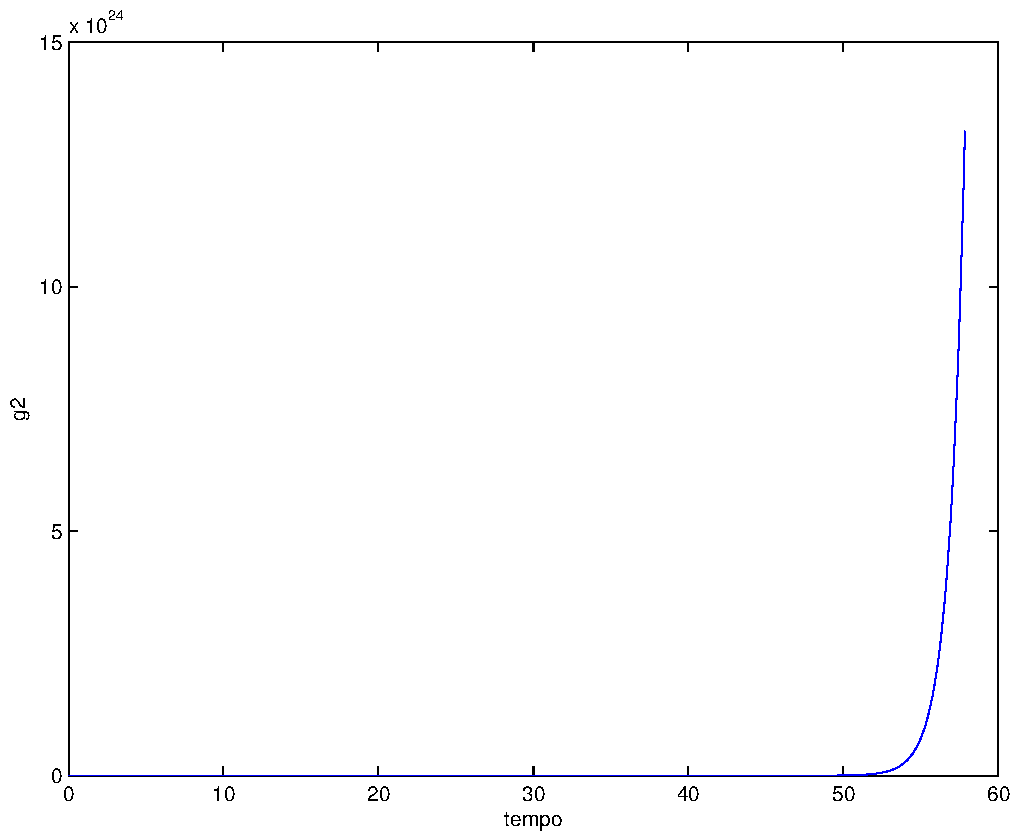
\includegraphics[scale=.5]{q1g2.pdf}
\end{center}

Nota-se que o valor de $g2$ cresce de forma exponencial e tente ao infinito, 
novamente por inspeção é possível concluir que o sistema é instável. Para
formalizar a conclusão, a figura abaixo mostra o plano-s,

\begin{center}
    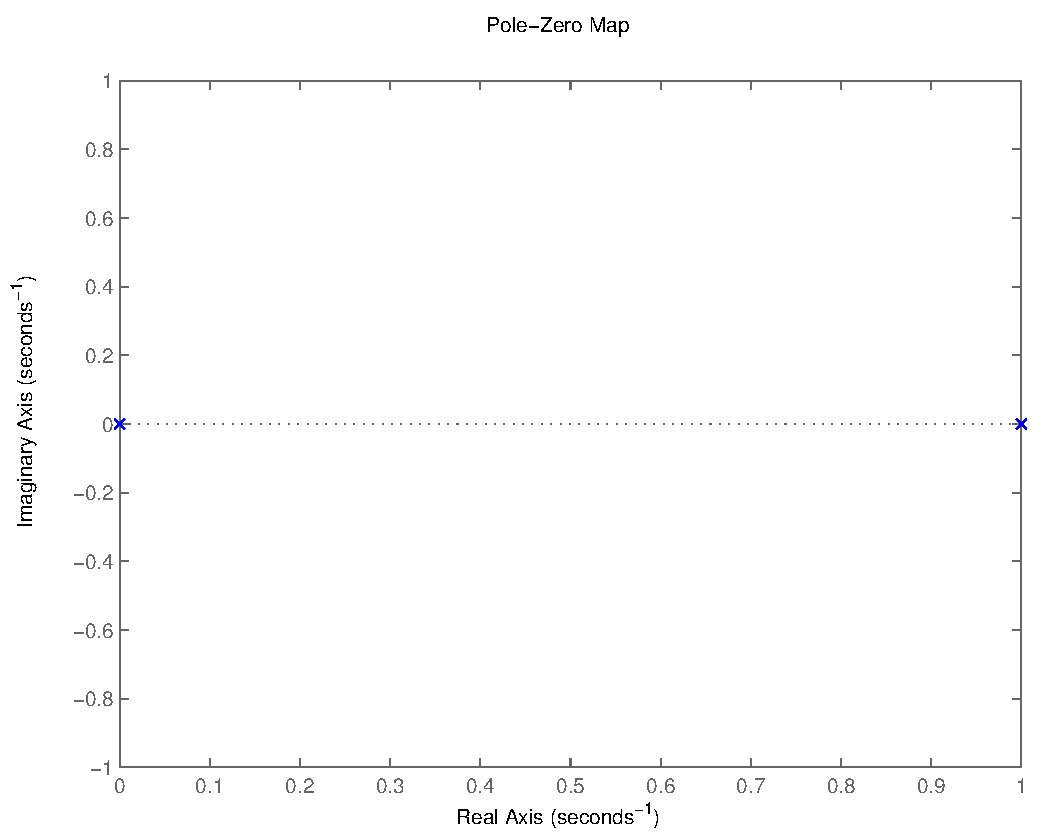
\includegraphics[scale=.5]{pzq1g2.pdf}
\end{center}

Nota-se que os polos são positivos e portanto na zona de instabilidade do plano-s.

Sobrepondo os dois gráficos da resposta temporal,

\begin{center}
    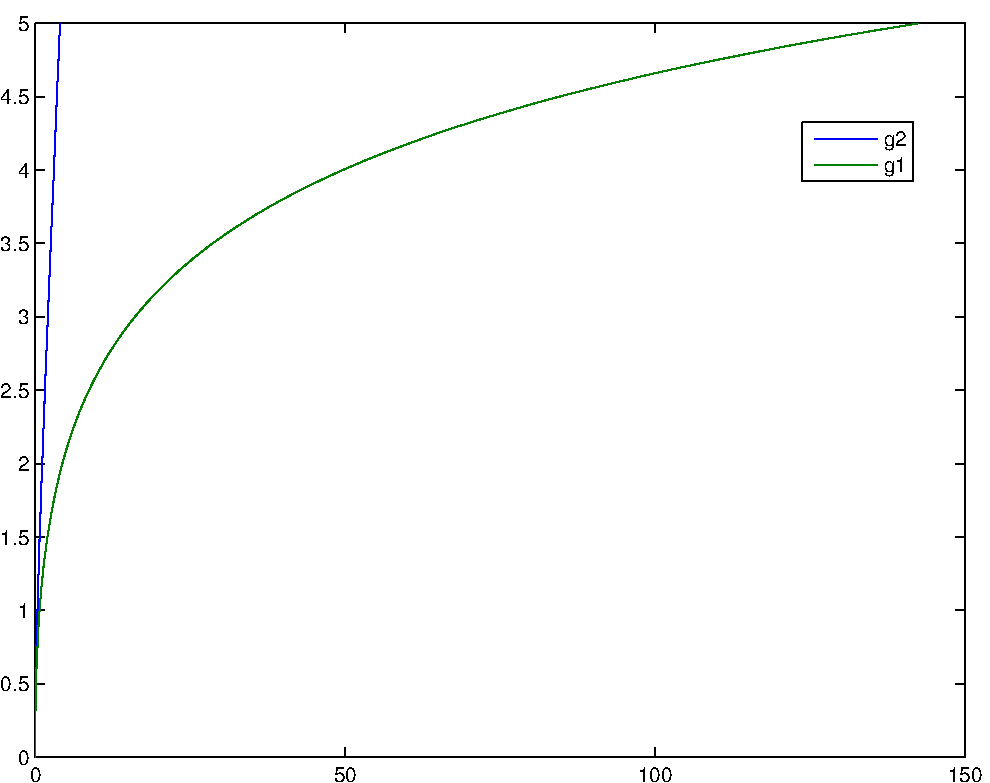
\includegraphics[scale=.5]{g1g2.pdf}
\end{center}

É possível visualizar que a função $g2$ cresce "infinitamente" mais rápida que $g1$
Finalmente é possível ver que a posição dos polos influencia facilmente a 
estabilidade de um sistema, é que o plano-s é uma ótima forma que visualizar
esta tal estabilidade, se contraponto até mesmo ao gráfico da resposta temporal.

%%%%%%%%%%%%%%%%%%%%%%%%%%%%%%%%%%%%%%%%%%%%%%%%%%%%%%%%%%%%%%%%%%%%%%%%%%%%%%%%
% SEGUNDA QUESTÃO
%%%%%%%%%%%%%%%%%%%%%%%%%%%%%%%%%%%%%%%%%%%%%%%%%%%%%%%%%%%%%%%%%%%%%%%%%%%%%%%%

\section{Segunda questão}

Para este problema foram propostos os seguintes sistemas,

\begin{center}
    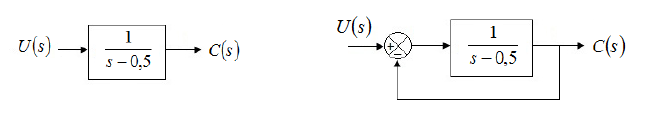
\includegraphics[scale=.5]{s2q.png}
\end{center}

\subsection{Analisando o sistema malha aberta}

O sistema de malha aberta tem a localização do polo mostrados na figura abaixo,

\begin{center}
    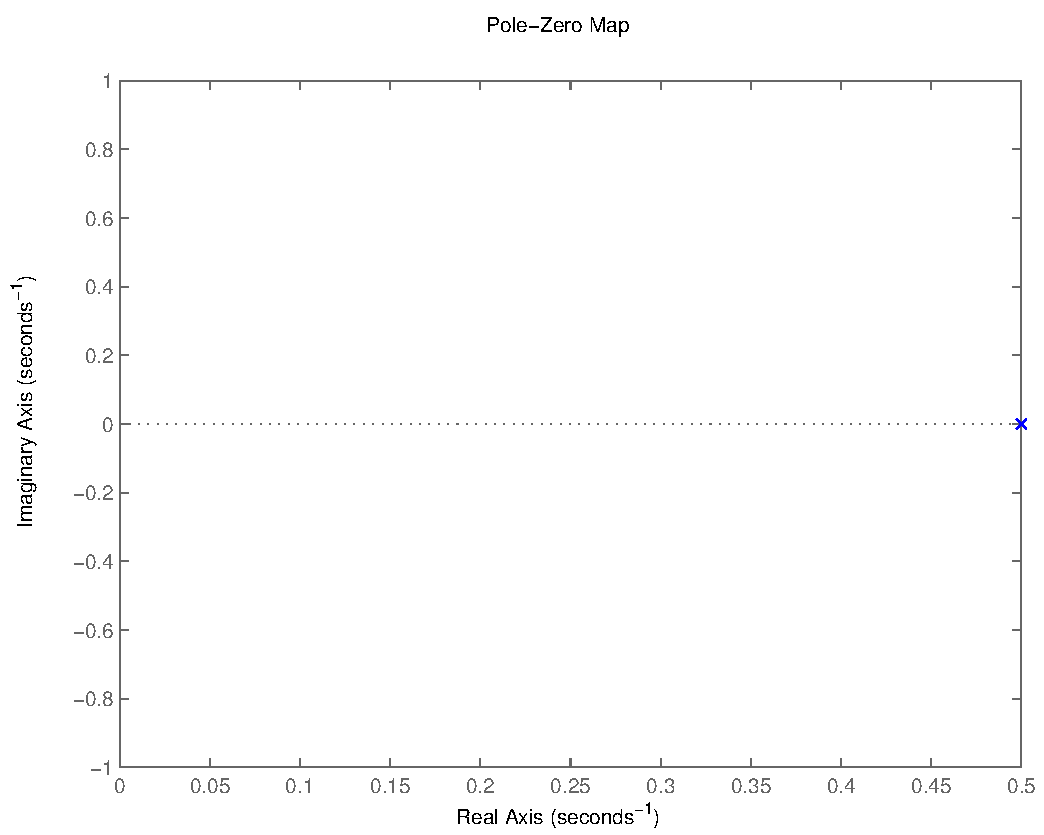
\includegraphics[scale=.5]{pz2qs1.pdf}
\end{center}

Mostrando claramente que o sistema apresenta uma instabilidade, está devida 
simplesmente a localização do polo.

\subsection{Analisando o sistema malha fechada}

A localização do polo é mostrado na figura abaixo,

\begin{center}
    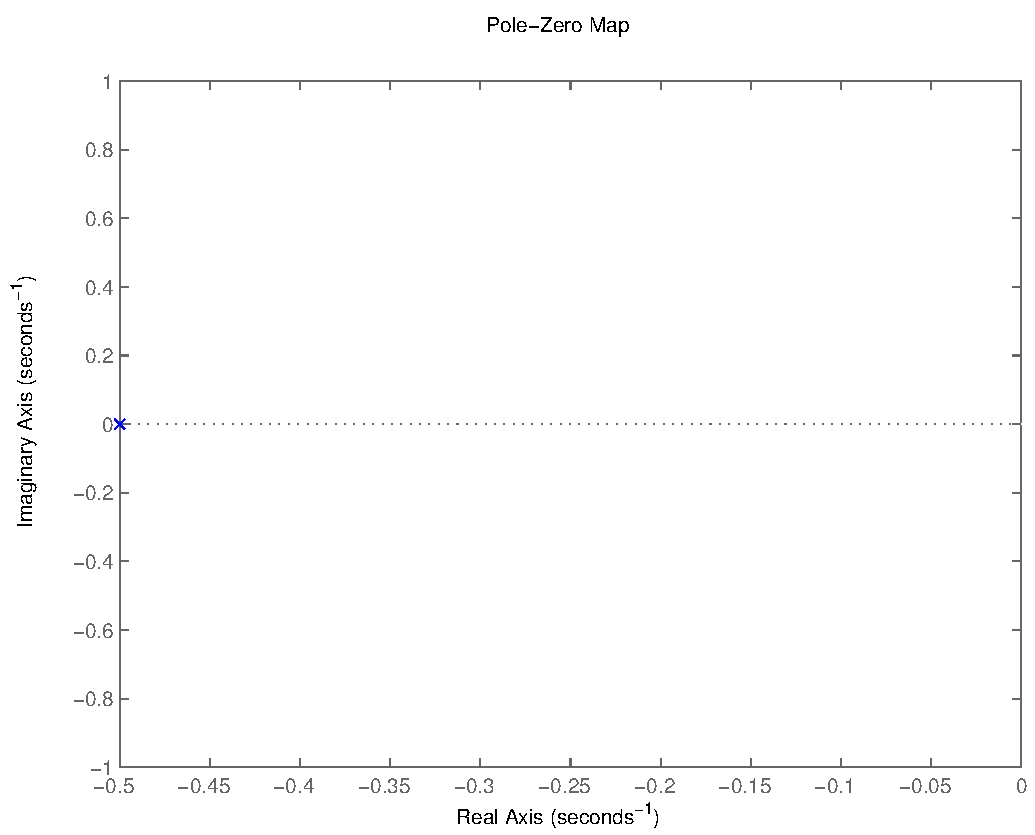
\includegraphics[scale=.5]{q2pzfechada.pdf}
\end{center}

Com a realimentação negativa e de ganho unitário pode ser visto que o sistema passou
de instável para estável.

\subsection{Efeitos da realimentação}

É possível concluir que o efeito da realimentação negativa em um sistema de controle
pode mudar a posição do polo, fazendo com que o mesmo passe para o lado esquerdo em
relação ao eixo imaginário, caracterizando em um sistema estável. E mais, o ganho
unitário não muda o ganho final da função, provando que não só o controle de ganho
é possível mudar a região de estabilidade.

Para finalizar a conclusão do efeito da realimentação, é mostrado abaixo o gráfico da resposta
ao degrau unitário $\frac{1}{s}$ para o sistema com e sem realimentação,

\begin{center}
    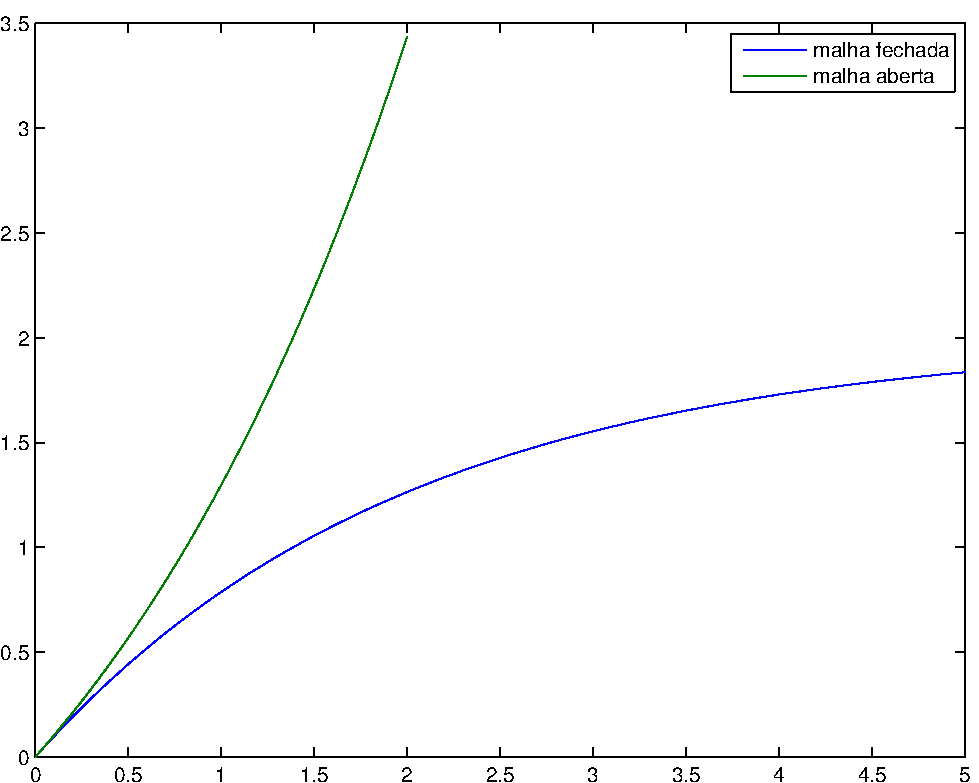
\includegraphics[scale=.5]{q2ib.pdf}
\end{center}

Como pode ser visto na figura a reposta em malha aberta ao degrau unitário 
tente ao infinito, contrastando com a resposta em malha fechada que em 
regime permanente é 2.

%%%%%%%%%%%%%%%%%%%%%%%%%%%%%%%%%%%%%%%%%%%%%%%%%%%%%%%%%%%%%%%%%%%%%%%%%%%%%%%%
% TERCEIRA QUESTÃO
%%%%%%%%%%%%%%%%%%%%%%%%%%%%%%%%%%%%%%%%%%%%%%%%%%%%%%%%%%%%%%%%%%%%%%%%%%%%%%%%

\section{Terceira questão}

O seguinte sistema de controle é proposto,

\begin{center}
    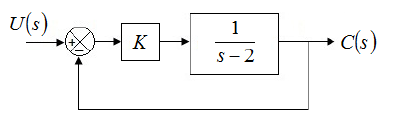
\includegraphics[scale=0.5]{q3.png}
\end{center}

Se faz necessário antes de iniciar a resolução dos itens do problema analisar o
sistema e seus comportamentos.

\subsection{Analisando o sistema\\Intervalo de $K$}

Para uma analise inicial, é possível fazer $K$ unitário, encontrando com isso a
função de transferência abaixo,

\begin{equation}
    \frac{1}{s-1}
\end{equation}

Esta função de transferência indica que o polo está em 1,com isto 
o sistema é instável. Para a correção desta instabilidade é possível
modificar o ganho, impondo que a condição aceitável para a estabilidade
no caso proposto é quando o polo fica no semi-plano esquerdo do plano-s, 
é possível então fazer,

\begin{equation}
    \frac{C(s)}{U(s)} = \frac{\frac{1}{s-2} K}{1 + \frac{1}{s-2} } = \frac{K}{K+s-2}
\end{equation}

Isolando $s$ do denominador de 9 para encontrar a posição do polo,

\begin{equation}
    s = - K + 2
\end{equation}

Com isto é possível concluir que o sistema só pode ser estável se $K$ for menor que 2.
Para o caso em que $K$ é igual a 2 o polo fica em 0.

\subsection{Gráficos em função de K}

O gráfico para quando $K_1=1$ e $K_2=3$ é mostrado abaixo,

\begin{center}
    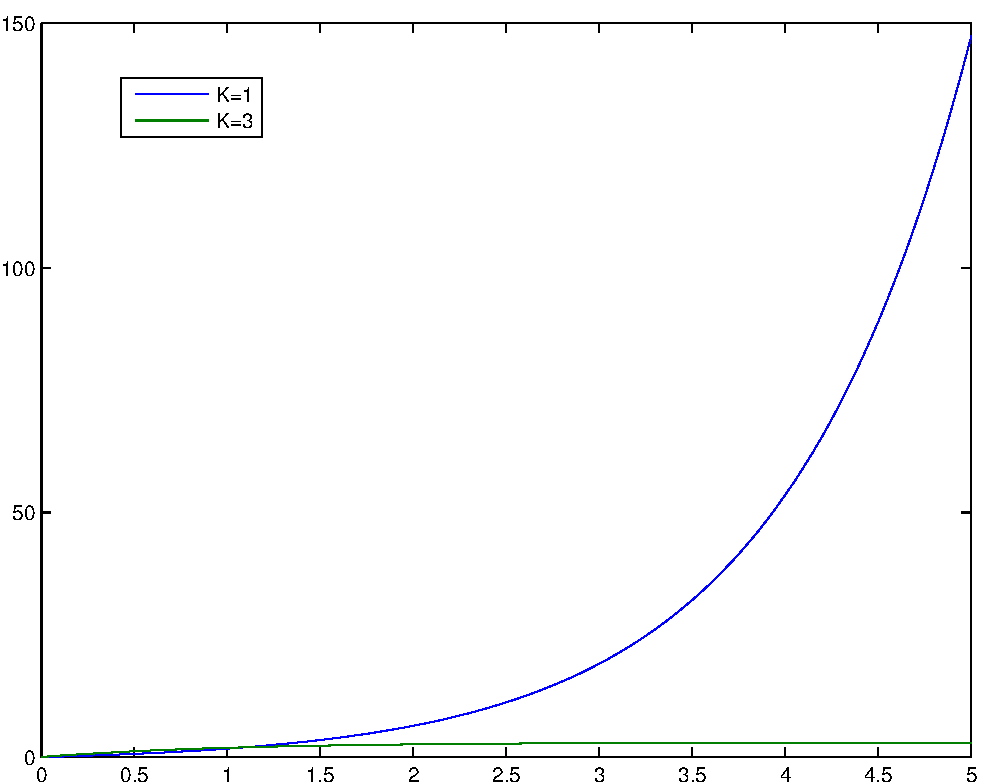
\includegraphics[scale=0.5]{q3ib.pdf}
\end{center}

O valor de $K$ é um fator interessante para o controle de estabilidade do um 
sistema de controle. Pois uma simples alteração pode fazer um sistema 
entrar em estabilidade. Mas com os devidos cuidados já que essa mesma alteração
pode resultar na destruição do projeto de controle.

\subsection{Conclusões finais sobre a estabilidade sistema de 1ª ordem}

Um sistema de primeira ordem é um dos mais simples para um sistema de controle, 
tanto em construção e principalmente na sua analise matemática. O controle
de ganho para os de 1ª ordem pode ser determinante no seu funcionamento. 
Para o problema da questão conclui-se que é possível não só

%%%%%%%%%%%%%%%%%%%%%%%%%%%%%%%%%%%%%%%%%%%%%%%%%%%%%%%%%%%%%%%%%%%%%%%%%%%%%%%%
% QUARTA QUESTÃO
%%%%%%%%%%%%%%%%%%%%%%%%%%%%%%%%%%%%%%%%%%%%%%%%%%%%%%%%%%%%%%%%%%%%%%%%%%%%%%%%

\newpage

\section{Quarta Questão}

Dois sistemas foram dados, o primeiro,

\begin{equation}
    G_1(s) = \frac{0.5}{s+0.5}
\end{equation}

e segundo,

\begin{equation}
    G_2(s) = \frac{5}{s+5}
\end{equation}

\subsection{Constante de tempo para os sistemas}

A equação temporal para o primeiro sistema quando submetido a um 
degrau unitário $u(t)=1$ em malha aberta é, no domínio da frequência fica,

\begin{equation}
    G_1(s) \frac{1}{s} = \frac{0.5}{s+0.5} \frac{1}{s} = \frac{0.5}{s^2 + 0.5 s}
\end{equation}
 
Expandindo em frações parciais,

\begin{equation}
    \frac{0.5}{s^2 + 0.5 s} = \frac{-1}{s+0.5} + \frac{1}{s}
\end{equation}

Aplicando a transformada inversa de Laplace

\begin{equation}
    g_1(t)=  -e^{-0.5 t} + 1
\end{equation}

Analisando agora o segundo sistema, da mesma forma que foi feita para o primeiro,

\begin{equation}
    G_2s) \frac{1}{s} = \frac{5}{s+5} \frac{1}{s} = \frac{5}{s^2 + 5 s}
\end{equation}
 
Expandindo em frações parciais,

\begin{equation}
    \frac{5}{s^2 + 5 s} = \frac{-1}{s+5} + \frac{1}{s}
\end{equation}

Aplicando a transformada inversa de Laplace

\begin{equation}
    g_2(t)=  -e^{-5 t} + 1
\end{equation}

A constante de tempo para os dois sistema informa algo interessante. A resposta
a um estimulo de entrada, para $G_1$ a constante de tempo é 2 e para $G_2$ é 
0.2, por inspeção se percebe que o sistema 2 é mais rápido do que o sistema 1.

\subsection{Localização dos polos}

Para o primeiro sistema a localização do polo é,

\begin{center}
    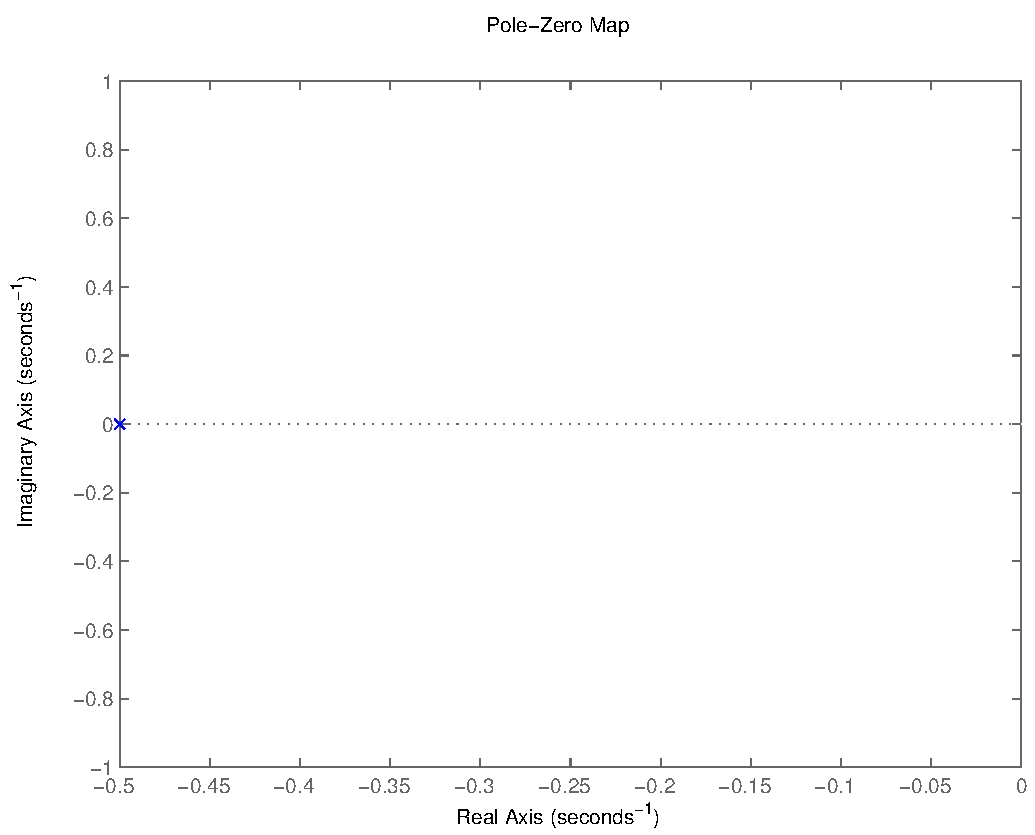
\includegraphics[scale=0.5]{q4pzg1.pdf}
\end{center}

Agora para o segundo sistema,

\begin{center}
    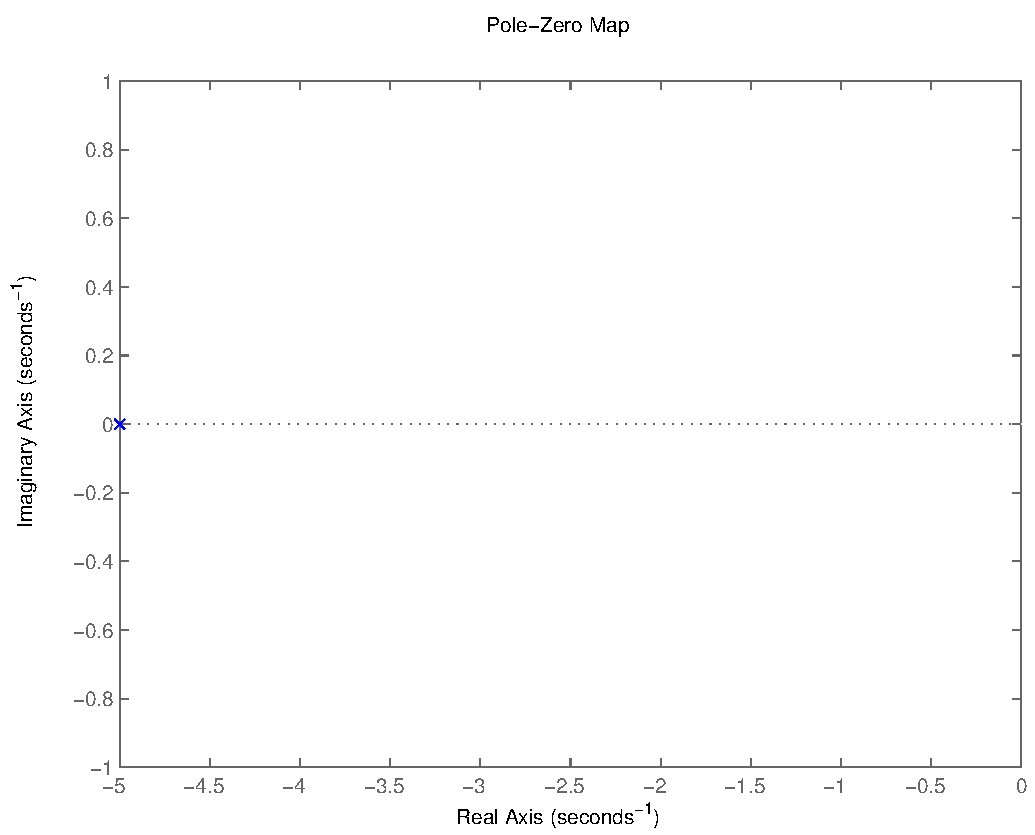
\includegraphics[scale=0.5]{q4pzg2.pdf}
\end{center}

Nota-se novamente que a localização dos polos alem de informa a estabilidade do sistema,
também informa o quanto é rápido a resposta dos sistemas a entrada. A primeiro sistema
o polo é localizado em 0.5 e o segundo sistema é 5, é possível com isto, concluir que
o sistema que tem um polo tendendo a menos infinito, ele é mais rápido.

\newpage

\subsection{Gráfico a resposta ao degrau}

Abaixo é mostrado o gráfico dos dois sistemas exemplificando novamente o que já foi 
dito anteriormente, $G2$ é mais rápido que $G1$

\begin{center}
    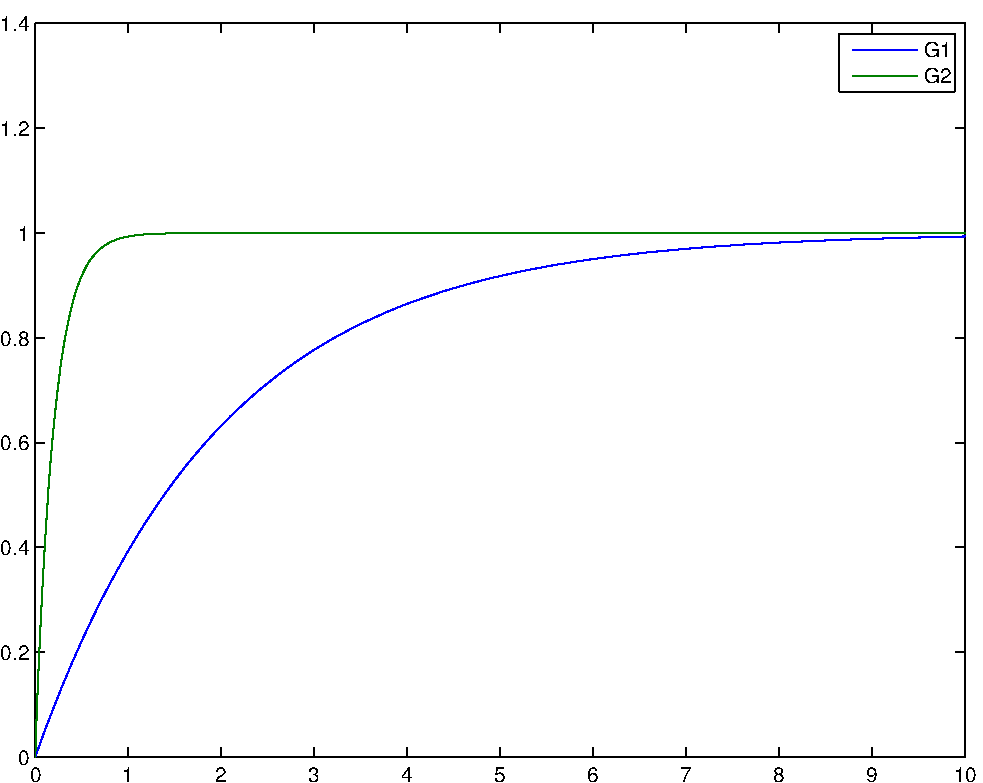
\includegraphics[scale=0.5]{q4ic.pdf}
\end{center}

\subsection{Conclusões finais}

BlaBla

\section{Quinta questão}

\begin{center}
    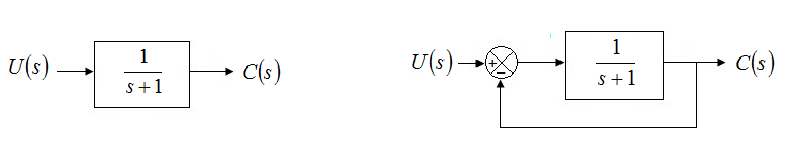
\includegraphics[scale=0.5]{q5.png}
\end{center}



\end{document}
